%!TEX root = ../report.tex
\chapter{Introduction}
\label{cha:Introduction}

In computer science, graphs are structures used for representing relationships between objects. A graph consists of vertices, sometimes called nodes, connected by edges, where the vertices represent the objects, and the edges represents the relationship. A graph can take on different shapes, giving the graph special properties. By giving the edges a direction the graph can take on further properties.

A graph where the edges have a direction is called a directed graph as seen in figure \ref{fig:DAG}. Here the vertices are connected to each other, with an arrow displaying the direction. An example of an undirected graph can be seen in figure \ref{fig:DAGvsAG}. In both types of graphs a vertex can have multiple edges. Graphs can contain cycles, meaning that vertices are connected to each other so that it is possible to follow edges in such a way that it leads back to the initial vertex. An example of such a cyclic graph can be seen in figure \ref{fig:DAGvsDG}. Acyclic graphs have an inherent topological ordering. This ordering makes it possible to find properties in the graph, such as the shortest path between two vertices.

\begin{figure}[h]
    \centering
    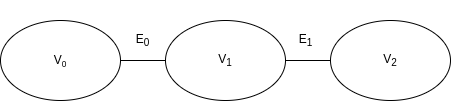
\includegraphics[scale=0.5]{figs/simpleAG.png}
    \caption{Example of non-directed graph.}
    \label{fig:DAGvsAG}
\end{figure}

\begin{figure}[h]
    \centering
    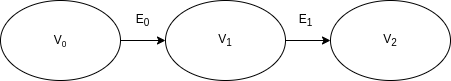
\includegraphics[scale=0.5]{figs/simpleDAG.png}
    \caption{Simple Directed graph.}
    \label{fig:DAG}
\end{figure}

\begin{figure}[h]
    \centering
    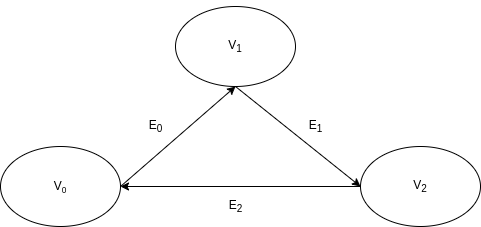
\includegraphics[scale=0.5]{figs/triangleDG.png}
    \caption{Directed graph with a cycle.}
    \label{fig:DAGvsDG}
\end{figure}

When using graphs as a form of storage, the vertices hold data, and the edges can be given an extra property describing the relation. Combining such a data store with common traversal methods for graphs results in an efficient extraction model for relational data. Some common traversal methods include breadth first search, where all neighboring vertices are discovered before moving on to the children of the currently discovered vertices. This contrasts to depth first search, where the children of a vertex is visited as they are discovered.

Databases using graphs have been created to overcome some of the limitations in traditional relational databases. Comparing such graph storage to relational storage, graph storage generally outperforms relational storage on structural queries, but not on data queries \cite{AComparisonOfGraphAndRelDB}. structural queries reference the graph structure, or the relationships in the data, while data queries look for specific data. When creating a graph database, an indexing system can also added. Such a system is ``Neo4j''\footnote{https://neo4j.com/} that use Apache Lucene\footnote{https://lucene.apache.org/} for indexing.

Another model for storing graph data is the Resource Description Framework (RDF). RDF often have its own form of storage, a ``triplestore'' based on the structure of the data. In RDF data is stored as triples, where a triple have the structure ``subject-predicate-object''. In this structure the subject and object can be considered vertices, and the predicate is the edge. In addition to forming the relation between the two vertices, the predicate also holds a type of relation. This makes it possible to apply reason to the data set, and derive new information from what is already there.

There are a few projects using RDF as an information storage system. Some of the more well known are DBPedia\cite{dbpedia}, YAGO\cite{yago}, and Creative Commons. These applications often consists of a large linked data set, or in the case of Creative Commons, it is used for embedding licenses. Creating methods that allows for easy access to information in RDF data makes it possible to create applications with utility. In this thesis methods for efficient keyword search on spatial and temporal data will be explored.

\section{Background and Motivation}
\label{sec:BackgroundAndMotivation}
UMost of the information on the web is unstructured, or semi-structured data. Using metadata and bots to help create structures can help both humans and computers. This is one of the goals of RDF. Creating ways for humans to discover data in new ways can create utility. To be able to get mor utility out of RDF, making it more accessible to humans needs to be done. Because of the highly linked nature of data that exists now, using these links can help provide that utility. As more data is generated, there are also more relations between the data. Exploring these relations can be done by using RDF or other graphs, but for a regular person this can be difficult. By proving that fast and accurate keyword search of spatiotemporal RDF graphs is possible new utilities for exploration can be built.


\section{Goals and Research Questions}
\label{sec:Goals and Research Questions}
\begin{description}
    \item[Goal] {\em This thesis has the goal of researching methods for spatiotemporal keyword searches on large RDF graphs, and what aspects needs to be considered for speed and accuracy.}
\end{description}
% Why this goal
Accomplishing this goal proves that RDF graphs can be used as a tool for structuring data related to real world places. There is a lot of data that can be placed at one or more real locations, either directly, or indirectly. By using RDF graphs it is possible to model how different places are connected through some pice of data, and how different pieces data can be related to real places.

\begin{description}
    \item[Research question 1] {\em How can spatiotemporal data be integrated into existing keyword query methods for RDF data?}
\end{description}
Extending existing methods for searching RDF data can make it simpler to search spatiotemporal data. By combining methods for temporal and spatial search, methods for spatiotemporal search should be possible to research.

\begin{description}
    \item[Research question 2] {\em What methods can be used to achieve greater speed and accuracy for searches on RDF data?}
\end{description}
An important aspect of any search is speed and accuracy. Since searching in graphs usually entails some form of traversal, the methods of traversal, as well as factors that affect speed and accuracy will be researched.

\begin{description}
    \item[Research question 3] {\em How do spatial and temporal RDF query methods differ from from other query methods?}
\end{description}
Comparing spatial, temporal and spatiotemporal searches can tell how spatiotemporal data differs in RDF graphs. This is important so that optimized methods can be developed.

\section{Research Method}
\label{sec:researchMethod}
This thesis will build on previous keyword search approaches for RDF graphs, and determine what methods can be expanded to incorporate spatiotemporal queries. A method for spatiotemporal search will be created, and methods for improvement will be tested, with the goal of finding what aspects of the search method have most effect for speed and accuracy.

\glsresetall